\documentclass[11pt]{article}
\usepackage{color,amsmath,amsfonts,amssymb,amsthm}

\usepackage[pdftex]{graphicx}
\DeclareGraphicsExtensions{.pdf, .jpg, .tif, .png}
\usepackage{rotating}

\textwidth=7.0in
\textheight=9.8in
\topmargin=-0.5in
\headsep=0.0in
\headheight=0.0in
\oddsidemargin=-0.25in
\evensidemargin=-0.25in

\begin{document}
{\bf Proposed repository workflow for MPAS cores within LANL.}\\
December 12, 2014\\
Mark Petersen\\

{\bf Requirements}
\begin{enumerate}
\item Upon completion, a new feature may be labeled as releasable or private.
\item Releasable features will be available to the public in the next release that the core participates in.
\item Private features will be available on the private branch, which is for LANL use only.
\item A development branch will be provided, which includes all releasable features.  
\item The development branch must be ready to release at any time.
\item A private branch will be provided for simulations internal to LANL, which includes both private and releasable features.
\item When private features are deemed releasable, they may be added to the development branch.
\item The private branch will occasionally be synchronized with the development branch, so that the private branch does not drift too far.  Ideally, the private branch is identical to the development branch, but with all private features added in.
\item Simulations for publications should be conducted on a permanent hash (a state the will be in the repository indefinitely).  We can't require this, but the the functionality should be there in the repository.
\item ACME can only point to a permanent hash.
\item The ability to release one feature should not depend on the private/releasable status of any other feature.
\item The ACME repository can only point to an MPAS-Core hash that can be public when ACME is eventually released.
\item ACME may be changed locally to point to other MPAS-core hashes.  These must be permanent hashes, and may be future-releasable or forever-private branches.
\end{enumerate}

\clearpage

Developer: designs, codes, and tests new features.  Responsible for their own feature branches.

Maintainer: developer, plus responsible for shared branches (release, development, and private branches)\\

{\bf Workflow:}\\

 \begin{tabular}[c]{l|l}
{\bf developer} & {\bf maintainer} \\
\hline 
 Start a new feature & \\
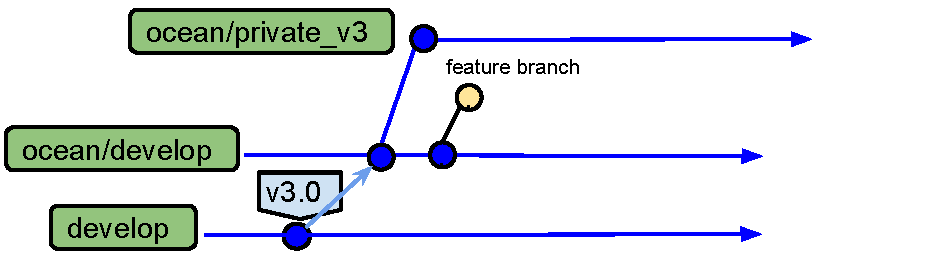
\includegraphics[width=3.5in]{f/MPASworkflow_1.pdf}& \\
\verb| git checkout MPAS-Dev/ocean/develop | & \\
\verb| git branch --no-track my_branch|  & \\
\verb| git push my_fork my_branch|  & \\
\hline 
 Commit changes to feature & \\
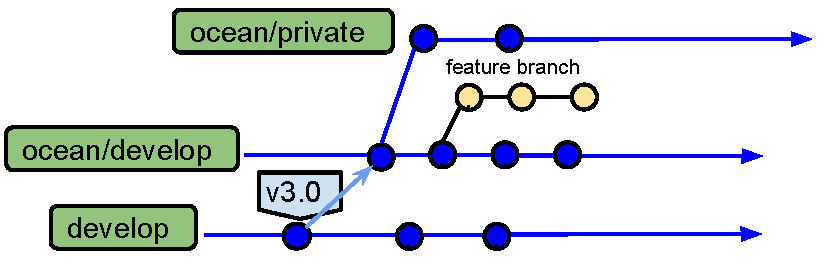
\includegraphics[width=3.5in]{f/MPASworkflow_2.pdf}& \\
\hline 
 Completion of releasable feature & \\
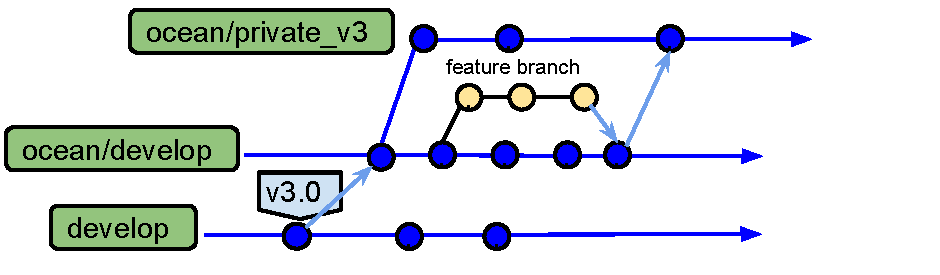
\includegraphics[width=3.5in]{f/MPASworkflow_3.pdf}& \\
\hline 
 Completion of private feature & \\
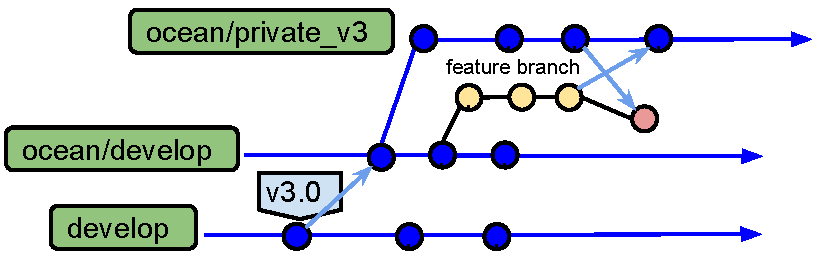
\includegraphics[width=3.5in]{f/MPASworkflow_4.pdf}& \\
\hline 
 Alterations of releasable feature after completion & \\
\hline 
 Alterations of private feature after completion & \\
\hline 
 Feature changes from private to releasable & \\
\hline 
 Keep private branched synchronized with & \\
 development branch  & \\
 \end{tabular}

%  \begin{tabular}[c]{c|c}
% \hspace{3in} & \hspace{3in}\\
% developer & maintainer 
%  \end{tabular}
% \begin{enumerate}
% \item Start a new feature \\
%  \begin{tabular}[c]{c|c}
% \hspace{3in} & \hspace{3in}\\
% developer & maintainer 
%  \end{tabular}
% \item Commit changes to feature & \\
% \item Completion of releasable feature
% \item Completion of private feature
% \item Alterations of releasable feature after completion
% \item Alterations of private feature after completion
% \item Feature changes from private to releasable
% \item Keep private branched synchronized with development branch 
% \end{enumerate}





% \begin{figure}[btp]
% \centering
% \begin{tabular}[c]{cccc}
% & tracer & layerThickness & maxLevelCell \\
% \begin{sideways}\hspace{0.2in}  bottom layer \end{sideways}&
% \includegraphics[height=1.5in, clip,trim=0 0 0 0]{f/c24u/c24u_DOME_temperature_b_20days_zoom.pdf} &
% \includegraphics[height=1.5in, clip,trim=0 0  0 0]{f/c24u/c24u_DOME_avgLayerThickness_b_20days_zoom.pdf}&
% \includegraphics[height=1.5in, clip,trim=0 0  0 0]{f/c24u/c24u_DOME_maxLevelCell_2_20days_zoom.pdf}\\
% \begin{sideways}\hspace{0.2in}  bottom layer-1 \end{sideways}&
% \includegraphics[height=1.5in, clip,trim=0 0 0 0]{f/c24u/c24u_DOME_temperature_B_20days_zoom.pdf} &
% \end{tabular}
% \caption{\label{fig:T striping zoom}
% {\bf 20 days instantaneous} DOME overflow cases, 15m layers, PBCs, zoom on striping.
% }
% \end{figure}

\end{document}


